\documentclass[10pt,a4paper]{beamer}
%\usepackage[utf8]{inputenc}
\usepackage[T1]{fontenc}
\usepackage[nynorsk]{babel}
\usepackage{amsmath}
\usepackage{amssymb}
\usepackage{graphicx}

\usepackage{svg}

\usepackage{import}

\usepackage{multicol}

\usetheme{metropolis}

\setbeamertemplate{section in toc}[sections numbered]
\setbeamertemplate{subsection in toc}[subsections numbered]

\usepackage[pagewise]{lineno}
\usepackage{csquotes}

\usepackage{minted}
\usepackage{listings}

\usepackage{multirow}

\usepackage{siunitx}
\usepackage{steinmetz}

\usepackage{xcolor}

\usepackage{enumerate}

\usepackage{lipsum}

\usepackage{caption}
\usepackage{subcaption}

\title{Grunnleggande innføring i \LaTeX}
\date{\today}
\author{Eirik Haustveit}
\institute{Institutt for datateknologi, elektroteknologi og realfag}
\begin{document}
	
	\titlepage
	
	\section{Historie}
	\label{sec:history}
	
	\begin{frame}{\TeX}
		
		I 1978 lanserte Donald Knuth eit typesettingssystem som han kalte for \TeX{}. Motivet hans for utvikling av \TeX{} var at han ønskte eit betre system for å skriva dei bøkene han jobba med.
		
		Formålet med \TeX{} var (og er) at kven som helst med rimelig enkelthet skulle kunne produsera bøker med høg kvalitet (typografisk sett).
		
		Namnet \TeX{} kjem frå gresk \(\tau\epsilon\chi\nu\eta\) som tyder ferdighet eller kunst. Den siste bokstaven i \TeX{}, $\chi$ er ein stor ``chi'', og uttalen av ordet \TeX{} er ``tekh''.
		
	\end{frame}
	
	\begin{frame}{\LaTeX}
		
		\includesvg[width=1.5in]{img/latex-project-logo.svg}
		
		\TeX{} kan vera ganske tungvindt å nytta direkte, og gir brukaren litt for mykje fleksibiliet i å styra utforminga av dokumentet. Når ein skriv eit dokument er det normalt ynskjeleg at dokumentet fylgjer ein gitt standard for typografi utan at ein manuelt må passe på dette.
		
		\LaTeX{} er ein utvidelse av \TeX{} med ulike tillegg som skal gjera det enklare å utarbeida dokument i henhold til ein gitt standard. Dvs. med ein gitt skrifttype, gitte margar, linjeavstandar og andre parameter som det er naturleg at skal vera konsekvent gjennom heile dokumentet. Ulike malar er tilgjengeleg for ulike dokumenttypar, og det er også mogleg å laga sin eigen mal.
		
	\end{frame}
	
	\section{Introduksjon til \LaTeX}
	
	\begin{frame}{Bruksområde for \LaTeX}
		
		\begin{itemize}
			\item Artiklar, rapportar, bøker m.m.
			\item Presentasjonar
			\item Typesettig av matemtaikk for import i andre program
			\item Teikning av figurar og grafar
		\end{itemize}
		
	\end{frame}


	\begin{frame}{\LaTeX vs Microsoft Word}
		
		Microsoft Word (og mange andre som til dømes Libre Office) er såkalla ``what you see is what you get'' (WYSIWYG) tekstredigeringsprogram. Det du ser ved redigering er det samme som det endelige resultatet. Det meste av funksjonaliteten er tilgjengeleg i menyar, men det betyr ikkje nødvendigvis at det er enkelt å finna fram til ein gitt funksjon.
		
		\LaTeX er eit ``what you see is what you mean'' (WYSIWYM) tekstredigeringssystem. Ein markerer teksten med spesielle kommandoar for å angi meininga, og så er det opp til \LaTeX å tolke denne meininga og presentera resultatet. Til dømes får ein \textbf{utheva tekst}, ved hjelp av markeringa \mintinline{latex}|\textbf{utheva tekst}|
		
		Det er truleg enklare å komma i gang med Word enn \LaTeX, og dette er kanskje ein viktig grunn til at det er så utbredt.
		
	\end{frame}
	
	\begin{frame}{Skyløysingar}
		
		Det er fleire ulike skyløysingar tilgjengelig for å skriva i \LaTeX. Ulempen med slike løysingar er først og fremst at ein legg alle filane sine på nokon andre si datamaskin. Ein anna ulempe er at det kan vera litt treigare og at det ikkje alltid er oppdatert til siste versjon av \LaTeX.
		
		Ei populær skyløysing er Overleaf: \url{https://www.overleaf.com/}. Dersom du ikkje har installert programvaren før oppmøte på kurset i dag så kan du oppretta ein brukar her for å testa ut det som vert demonstrert.
		
	\end{frame}
	
	
	\begin{frame}{Installasjon av programvare}
		
		Framgangsmåten for installasjon av \LaTeX{} vil variera avhengig av kva operativsystem ein nyttar.
		
		For Windows kan ein installera MikTeX: \url{https://miktex.org/download}.
		
		Ein treng også ein teksteditor, og her er TeXstudio eit godt alternativ: \url{https://www.texstudio.org/}
		
		Brukarar av MacOS, eller Linux kan også nytta MikTeX, men har også andre alternativ. Bruk google, eller spør om hjelp om du ikkje finn ut av det sjølv.
	\end{frame}
	
	\section{Bruk av \LaTeX}
	
	\begin{frame}{Introduksjon}
		
		Eit \LaTeX{} dokument består av ein eller fleire kjeldefilar (*.tex) som vert lest av ein kompilator og konvertert til eit dokument, vanlegivis i *.pdf format.
		
		Programmet som les *.tex filane er ein vanleg programfil utan grafisk brukargrensesnitt (konsollprogram). Ein har ulike alternativ:
		
		\begin{itemize}
			\item pdflatex
			\item XeLaTeX
			\item LuaLaTeX
		\end{itemize}
		
	\end{frame}
	
	
	\begin{frame}{Introduksjon}
	
	For å redigera kjeldefilane i eit \LaTeX{} dokument treng ein eit tekstredigeringsprogram. TeXstudio er eit program som er speisallaga for å skriva \LaTeX{}, og har ein del innebygd funksjonalitet for å gjera dette enklare.
	
	I staden for å skriva kommandoen \mintinline{console}|pdflatex bachelorrapport.tex| kan ein trykka på den grøne pilen i TeXstudio for å bygga dokumentet.

	\end{frame}
	
	\begin{frame}[containsverbatim]{Oppbygging av eit dokument}
		
\begin{minted}{latex}
\documentclass[10pt,a4paper]{article}
%\usepackage[utf8]{inputenc} % Ikkje for LuaLaTeX
\usepackage[T1]{fontenc}
\usepackage[nynorsk]{babel}

\author{Eirik Haustveit}
\title{Demo}
\begin{document}
	Eit enkelt dokument
\end{document}
\end{minted}
		
	\end{frame}
	

	\begin{frame}[containsverbatim]{Oppbygging av eit dokument}
	
	Koden før \mintinline{latex}|\begin{document}| vert kalla ``preamble''. Her importerer ein pakkar som tilbyr ekstra funksjonalitet og endrer instillingar som gjeld heile dokumentet.
	
	Mellom \mintinline{latex}|\begin{document}| og \mintinline{latex}|\end{document}| plasserer ein alt innhaldet i dokumentet. Dette inkluderer den reine teksten ein jobbar med, samt kommandoar som markerer teksten for å oppnå dei tilpassingane ein ynskjer.
	
	\mintinline{latex}|\usepackage[utf8]{inputenc}| velger at teksten som \LaTeX{} får inn (den teksten du skriv) skal tolkast som UTF-8. Denne pakken er ikkje nødvendig i dei moderne kompilatorane XeLaTeX, og LuaLaTeX.
	
	\mintinline{latex}|\usepackage[T1]{fontenc}| velger kva type skriftkoding (font encoding) som skal nyttast. Dette er ikkje det samme som å velga skrifttype. Denne pakken er nesten alltid med.
	
	\end{frame}
	
	
	\begin{frame}{Inndeling i seksjonar og kapittel}
		
		Inndeling av dokumentet i kapittel og underkapittel (seksjonar) vert gjort med ulike kommandoar avhengig av nivået:
		
		\mintinline{latex}{\section{tittel}}, \mintinline{latex}{\subsection{tittel}}, \mintinline{latex}{\subsubsection{tittel}}
		
		\mintinline{latex}{\chapter{tittel}}
				
	\end{frame}

	\begin{frame}{Feilmeldingar}
	
	Dersom du skriv ein ugyldig kommando vil du få ein feilmelding på samme måte som ved kompilering av eit program. Det er ulike kategoriar av feilmeldingar, nokon vil stoppa bygginga av dokumentet, medan andre berre fordel deg at noko er galt og at dokumentet truleg ikkje vil sjå ut slik som du hadde tenkt.
	
%	\begin{itemize}
%		\item error
%		\item warning
%		\item bad box
%	\end{itemize}
	
	Det er viktig at ein sjekker feilloggen regelmessig, og at ein håndterer eventuelle feilmeldingar etter kvart. Dersom det hopar seg opp med ``warnings'' så kan det vera mykje arbeid å finna ut av ein feil når det til slutt ikkje fungerer lenger.
	
	\begin{figure}
		\centering
		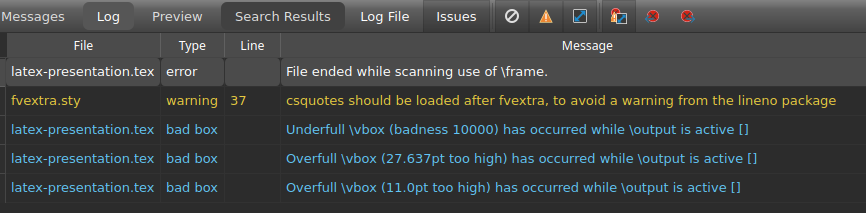
\includegraphics[width=0.9\linewidth]{img/latex-error-example}
		\caption{Døme på feilmeldingar i TeXStudio}
		\label{fig:latex-error-example}
	\end{figure}
	
	
	\end{frame}
	
	\begin{frame}{Dokumentklassar}
		
		\LaTeX{} har ein del innebygde dokumentklassar, og det er også mulig å lasta ned fleire, eller laga sine eigne. Nokon av dei viktigaste er:
		
		\begin{itemize}
			\item article - korte rapportar, dokumentasjon, vitskaplig artikkel m.m.
			\item report - For lengre rapportar, avhandlingar og korte bøker
			\item book - For bøker
			\item letter - For brev
			\item beamer - For presentasjonar
		\end{itemize}
		
	\end{frame}
	
	\begin{frame}{Innhaldsfortegnelse}
		
		Ei innhaldsfortegnelse i \LaTeX{} vert normalt autogenerert ut frå inndelinga i seksjonar og kapittel. Kommandoen \mintinline{latex}{\tableofcontents} plasserer innhaldsfortegnelsen der ein måtte ynskja, til dømes her:
		
		\tableofcontents
	\end{frame}
	
	\begin{frame}{Fotnoter}
		
		Ei fotnote er eit notat til ein tekst plassert nederst på sida, med eit teikn i brødteksten som refererer til fotnoten\footnote{Fotnoter er ofte nytta som eit alternativ til å inkludera ei lang forklaring inne i brødteksten. Ein lesar som forstår teksten kan då hoppa over fotnoten, medan ein som har problem med å forstå teksten kan få hjelp.}. Kommandoen for å setta inn ei fotnote må plasserast der ein ynskjer å plassera referansen:
		
		\mintinline{latex}{..refererer til fotnoten\footnote{Fotnoter er ofte...}.}
		
	\end{frame}
	
	\begin{frame}{Kryssreferansar}
		
		Kryssreferering er interne referansar i eit dokument for å fortelja lesaren kvar han kan finna gitt informasjon i dokumentet. Til dømes:
		
		\begin{displayquote}
			Ohms lov er gitt i formel \eqref{eq:ohms-law}. Bla bla bla, meir tekst.... meir tekst meir tekst
			
			\begin{equation}
				U = R \cdot I
				\label{eq:ohms-law}
			\end{equation}

		\end{displayquote}
		
		Eit anna relevant døme er:
		
		\begin{displayquote}
			Grunnleggande om historien til \TeX og \LaTeX er gitt i avsnitt \ref{sec:history}.
		\end{displayquote}
		
	\end{frame}
	
	
	\begin{frame}[containsverbatim]{Listing av kjeldekode}
		
		Kjeldekode i ulike programmeringsspråk vert normalt lista i ulike fargar for betra lesbarheten.
		
		Til dømes i Matlab:
		
\begin{minted}{matlab}
% Generate a random number
a = randi(100, 1);

% If it is even, divide by 2
if rem(a, 2) == 0
disp('a is even')
b = a/2;
end
\end{minted}

	\end{frame}




	\begin{frame}[containsverbatim]{Listing av kjeldekode}
		Ein har ulike pakkar for listing av kjeldekode.
		
		\begin{itemize}
			\item verbatim
			\item listings
			\item Minted
		\end{itemize}
	
	Den mest avanserte (beste?) er Minted, men den krever at ein har installert Python. Dersom ein ikkje har avanserte behov kan ein nytta listings.

\begin{lstlisting}
\begin{minted}{latex}
	
\end{minted}
\end{lstlisting}

	\end{frame}


	\begin{frame}[containsverbatim]{Importering av eksterne filar}
	
	Importering av eksten kjeldekode gjer det enklare å holda dokumentet oppdatert. Endringar i den kjeldekoden du jobbar med vil umiddelbart bli reflektert i rapporten som skal dokumentera koden:

\begin{minted}{latex}
\inputminted[<options>]{<language>}{<filename>}
\end{minted}
	
	Til dømes vil \mintinline{latex}|\inputminted{csharp}{source-code/hello.cs}| i denne presentasjonen gi oss:
	
	\inputminted{csharp}{source-code/hello.cs}
	
	\end{frame}
	
	
	\begin{frame}[containsverbatim]{Matematikk}
		
		Dersom ein jobbar med ingeniørfag vil det ofte vera behov for å beskriva matematiske uttrykk. Det er derfor viktig å ha eit fleksibelt og enkelt system for dette. Dette er ein av dei største styrkene til \LaTeX, og det er faktisk mulig å nytta den samme syntaksen for å setta inn formlar i Microsoft Word. For å typesetta fylgjande uttrykk:
		
		\begin{equation}
			\int_0^\infty \mathrm{e}^{-x}\,\mathrm{d}x
		\end{equation}
		
		Kan ein nytta fylgjande kode:
		
\begin{minted}{latex}
\begin{equation}
\int_0^\infty \mathrm{e}^{-x}\,\mathrm{d}x
\end{equation}
\end{minted}
		
	\end{frame}



	
\begin{frame}[containsverbatim]{Matematikk}
	
	Dersom ein ikkje ynskjer nummerering kan ein skriva:
	
	\begin{minted}{latex}
\begin{equation*}
	\int_0^\infty \mathrm{e}^{-x}\,\mathrm{d}x
\end{equation*}
	\end{minted}
	
	For å plassera matematikk inne i teksten kan ein nytta:
	
	\mintinline{latex}|\(a = \frac{b}{c}\)|, som gir: \(a = \frac{b}{c}\)
	
	Unngå bruk av dollarteikn (\$) sjølv om det også fungerer:
	\mintinline{latex}|$a = \frac{b}{c}$|, som gir: $a = \frac{b}{c}$

	Dollarteikn er ein \TeX{} kommando, og vil ikkje gi like gode feilmeldingar som \mintinline{latex}|\(\)| i \LaTeX{}.
	

	
\end{frame}



	\begin{frame}[containsverbatim]{Avansert matematikk}
		
\begin{equation}
	z = \overbrace{
		\underbrace{x}_\text{reell} + j
		\underbrace{y}_\text{lateral}
	}^\text{komplekst tal}
\end{equation}
	
	\begin{minted}{latex}
\begin{equation}
z = \overbrace{
	\underbrace{x}_\text{reell} + j
	\underbrace{y}_\text{lateral}
}^\text{komplekst tal}
\end{equation}
	\end{minted}

	\end{frame}


	\begin{frame}{Organisering av dokumentet i fleire filar}
		
		For å betra organiseringa av eit dokument og for å forenkla samarbeid kan det delast opp i fleire filar. Til dømes ein fil for kvart kapittel. \LaTeX støtter ulike kommandoar for innhenting av eksterne filar\footnote{Merk at det her er snakk om filar med \LaTeX-kode, ikkje kjeldekode som skal listast opp.}
		
		\begin{itemize}
			\item \mintinline{latex}|\input{vedlegg.tex}|
			\item \mintinline{latex}|\include{vedlegg.tex}|
			\item \mintinline{latex}|\import{vedlegg.tex}|
			\item \mintinline{latex}|\subfile{vedlegg.tex}|
		\end{itemize}
		
	\end{frame}

	\begin{frame}{Organisering av dokumentet i fleire filar}
		
		Forskjellen på \mintinline{latex}|\input{vedlegg.tex}|, og \mintinline{latex}|\include{vedlegg.tex}| er at den siste setter inn eit sideskift før og etter innhenting av den eksterne filen (kommandoen for å gjera dette manuelt er: \mintinline{latex}|\clearpage|).
		
		Kommandoen \mintinline{latex}|\import{vedlegg.tex}| er ikkje innebygd, og krever at ein legg til \mintinline{latex}|\usepackage{import}| i preamble.
		
		Det samme gjeld \mintinline{latex}|\subfile{vedlegg.tex}|, som krev \mintinline{latex}|\usepackage{subfiles}|
		
		%Import gjer det enklare å organisera større \LaTeX{} prosjekt. \mintinline{latex}|\subimport{}|
		
	\end{frame}

	\begin{frame}{Organisering av dokumentet med subfile}
	
	Ved hjelp av ``subfiles'' pakken kan du bygga kvar ekstern fil individuelt, og dei vil automatisk nytta samme ``preamble'' som hovudfilen.
	
	\end{frame}


	\begin{frame}{Skrifttypar og skriftstorleik}
	
	
	\url{https://tug.org/FontCatalogue/}
	
	
	\end{frame}

	\begin{frame}{Skriving på norsk}
	\mintinline{latex}|\usepackage[nynorsk]{babel}|
	
	\mintinline{latex}|\usepackage{parskip}|
	
	\end{frame}

	\begin{frame}[containsverbatim]{Kolonner}
		
		Dokumentet kan delast opp i kolonner ved hjelp av \mintinline{latex}|\usepackage{multicol}|
		
		\begin{columns}
	    	\begin{column}{0.49\textwidth}
			
\begin{minted}{latex}
\begin{multicols}{2}[]
the quick brown...
\end{multicols}
\end{minted}
				
		\end{column}
			% Column 2 (vertical line)
			\begin{column}{.02\textwidth}
				\rule{.1mm}{0.7\textheight}
			\end{column}
			% Column 3    
			\begin{column}{0.245\textwidth}
			The quick brown fox jumps over the lazy dog the quick brown fox jumps over the lazy dog	the quick brown fox jumps over the lazy dog
			\end{column}
			\begin{column}{0.245\textwidth}
			The quick brown fox jumps over the lazy dog	the quick brown fox jumps over the lazy dog the quick brown fox jumps over the lazy dog
			\end{column}
		\end{columns}

		
%		\begin{multicols}{3}
%			[
%			\section{First Section}
%			All human things are subject to decay. And when fate summons, Monarchs must obey.
%			]
%			test
%			fasfd
%		\end{multicols}
	
	\end{frame}

	\begin{frame}[containsverbatim]{Fargar}
	
	
	\color{red} Tekst \color{green} kan \color{blue} skrivast \color{purple} i \color{yellow} ulike \color{orange} fargar.
	
	{\color{red} \rule{\linewidth}{0.5mm}}
	
	\color{black}
	
	For å få til dette kan ein nytta \mintinline{latex}|\usepackage{xcolor}|
	
	\begin{minted}[breaklines]{latex}
\color{red} Tekst \color{green} kan \color{blue} skrivast \color{purple} i \color{yellow} ulike \color{orange} fargar.
	\end{minted}
	
	\end{frame}

	\begin{frame}[containsverbatim]{Punktlister og nummererte lister}
		
		\begin{itemize}
			\item Eit element
			\item Eit element til
		\end{itemize}
	
	\begin{minted}{latex}
\begin{itemize}
	\item Eit element
	\item Eit element til
\end{itemize}
	\end{minted}
		
	\end{frame}


	\begin{frame}[containsverbatim]{Punktlister og nummererte lister}
	
	\begin{enumerate}
		\item Eit element
		\item Eit element til
	\end{enumerate}
	
	\begin{minted}{latex}
\begin{enumerate}
	\item Eit element
	\item Eit element til
\end{enumerate}
	\end{minted}
	
	\begin{enumerate}
		\item[*] Eit element
		\item[!] Eit element til
		\item Enda eit
	\end{enumerate}
	
	\begin{minted}{latex}
\begin{enumerate}
	\item[*] Eit element
	\item[!] Eit element til
	\item Enda eit
\end{enumerate}
	\end{minted}
	
	\end{frame}


	\begin{frame}{Figurar (bilete)}
	
	Høgskulen sin logo er gitt i figur \ref{fig:hvl-logo}.
	
	\begin{figure}
		
\includegraphics[scale=0.1]{img/HVL-logo-vert-pos-norsk.png}
		\caption{HVL sin logo}
		\label{fig:hvl-logo}
	\end{figure}
	
	\end{frame}


	\begin{frame}[containsverbatim]{Figurar (bilete)}
	
	\begin{minted}[breaklines]{latex}
Høgskulen sin logo er gitt i figur \ref{fig:hvl-logo}.

\begin{figure}

\includegraphics[scale=0.1]{img/HVL-logo-vert-pos-norsk.png}
\caption{HVL sin logo}
\label{fig:hvl-logo}
\end{figure}
	\end{minted}
	
	\end{frame}

	\begin{frame}[containsverbatim]{Underfigurar}
		
		Det kan vera nyttig å gruppera ein figur i fleire underfigurar. Til dømes eit krinsskjema og ein graf som beskriv responsen til krinsen.
		
		\textbf{Ikkje bruk denne utdaterte pakken:} \mintinline{latex}|\usepackage{subfig}|. Den var sist oppdatert i 2005.
		
		I staden bør du bruka:
		
		\begin{minted}{latex}
\usepackage{caption}
\usepackage{subcaption}
		\end{minted}

		
	\end{frame}


	\begin{frame}[containsverbatim]{Underfigurar}
	
\begin{figure}
	\centering
	\begin{subfigure}[b]{0.3\textwidth}
		\centering
		\includegraphics[width=\textwidth]{example-image-a}
		\caption{Den første figuren}
		\label{fig:first-fig}
	\end{subfigure}
	\hfill
	\begin{subfigure}[b]{0.3\textwidth}
		\centering
		\includegraphics[width=\textwidth]{example-image-b}
		\caption{Den andre figuren}
		\label{fig:second-fig}
	\end{subfigure}
	\hfill
	\begin{subfigure}[b]{0.3\textwidth}
		\centering
		\includegraphics[width=\textwidth]{example-image-c}
		\caption{Den tredje figuren}
		\label{fig:third-fig}
	\end{subfigure}
	\caption{Tre figurar}
	\label{fig:three-figures}
\end{figure}
	
	Figur \ref{fig:first-fig} syner ein A, medan figur \ref{fig:second-fig} syner ein B.
	
	\end{frame}


	\begin{frame}[containsverbatim]{Underfigurar}
	
	\begin{minted}{latex}
\begin{figure}
\centering
\begin{subfigure}[b]{0.3\textwidth}
	\centering
	\includegraphics....
	\caption{Den første figuren}
	\label{fig:first-fig}
\end{subfigure}
\hfill
\begin{subfigure}[b]{0.3\textwidth}
	\centering
	\includegraphics....
	\caption{Den andre figuren}
	\label{fig:second-fig}
\end{subfigure}
...
\end{figure}
	\end{minted}

	
	
	
	\end{frame}


	\begin{frame}[containsverbatim]{Tabellar}
		
	Tabellar kan opprettast i ``tabular'' miljøet.
		
\begin{table}
	\caption{Teknisk tabell}
\begin{tabular}{ |c|c|c|c| } 
	\hline
	kolonne1 & kolonne2 & kolonne3 \\
	\hline
	\multirow{3}{4em}{Fleire rader} & celle2 & celle3 \\ 
	& celle5 & celle6 \\ 
	& celle8 & celle9 \\ 
	\hline
\end{tabular}
\end{table}

	\begin{minted}{latex}
\begin{tabular}{ |c|c|c|c| } 
\hline
kolonne1 & kolonne2 & kolonne3 \\
\hline
\multirow{3}{4em}{Fleire rader} & celle2 & celle3 \\ 
& celle5 & celle6 \\ 
& celle8 & celle9 \\ 
\hline
\end{tabular}
	\end{minted}

	\end{frame}

	\begin{frame}[containsverbatim]{Tabellar}
		
		For å laga litt finare tabellar kan ein nytta: \mintinline{latex}|\usepackage{booktabs}|.
		
	\end{frame}


	\begin{frame}{hyperref pakken}
	
	
	\end{frame}


	\begin{frame}{Referanselister}
		
		Skikkelige referanselister er både viktig for å unngå plagiat, og nyttig for å hjelpa lesaren til å finna meir informasjon. \LaTeX har ulike system for å automatisera delar av jobben med innhenting av metadata, og generering av referanselister:
		
		\begin{itemize}
			\item BibTeX
			\item BibLaTeX
		\end{itemize}
	
		BibLaTeX er det moderne alternativet til BibTeX og er det som bør nyttast.
		
	\end{frame}


	\begin{frame}{Referanselister}
	
	Ei referanse har ein del metadata som tittel, forfattar, publiseringsdato, ISBN nummer (for bøker), .m.m. Denne informasjonen vert lagt i eigne *.bib filar som BibLaTeX nyttar for å generera referanselistene. *.bib filane kan ein enten skriva manuelt, eller ein kan nytta ulike verktøy for å generera dei automatisk.	
	
	\end{frame}


	\begin{frame}{Referansehåndtering med Zotero}
	
	
	\end{frame}


	\begin{frame}{Måleeiningar}
		
		Pakken siunitx (\mintinline{latex}|\usepackage{siunitx}|) kan nyttast for å forenkla arbeidet med konsekvent typesetting av SI einingar.
		
		\mintinline{latex}|\(U = \SI{230}{\kilo\volt}\)| gir: \(U = \SI{230}{\kilo\volt}\)
		
		Fasevektorar kan typesettast ved hjelp av:
		\mintinline{latex}|\(\SI[parse-numbers=false]{38\phase{34^{\circ}}}{\ampere}\)|
		
		Som gir: \( \SI[parse-numbers=false]{38\phase{34^{\circ}}}{\ampere}\)
		
	\end{frame}


	\begin{frame}{Vidare lesing}
	
	Denne presentasjonen har forsøkt å gi ein introduksjon til grunnleggande \LaTeX{} for at ein skal komma i gang med skrivinga. Det er mange avanserte tema som ikkje er tatt med.
	
	\begin{itemize}
		\item Bruk av teljarar
		\item Generering av ordlister og symbollister
		\item Plotting av grafar med pgfplots
		\item Teikning av elektriske krinsar med circuitikz
		\item Generell tekning med TikZ
		\item Programmering i \TeX{}
		\item Utvikling av eigne malar og andre pakkar
	\end{itemize}
	
	
	\end{frame}

	\begin{frame}{Referansar}	
	
	
	
	\end{frame}
	
	
\end{document}